\documentclass[conference, final]{IEEEtran}

\IEEEoverridecommandlockouts

\usepackage{cite}
\usepackage{amsmath,amssymb,amsfonts}
\usepackage{algorithm}
\usepackage{algorithmicx}
\usepackage{graphicx}
\usepackage{textcomp}
\usepackage{xcolor}
\usepackage{bm}
\usepackage{multirow}
\usepackage{array}
\usepackage[noend]{algpseudocode}
\usepackage{subcaption}
\usepackage{url}


\usepackage{color}
\usepackage{xcolor,soul}
\usepackage{setspace}

\captionsetup[subfigure]{font=footnotesize,labelfont=footnotesize}
\DeclareMathOperator*{\argmin}{argmin}
\DeclareMathOperator*{\argmax}{argmax}


\newcommand{\hlb}[2][blue]{{\color{#1} {#2}}\unskip }


%These two commands fix the "top margin" error in IEEE submission 
% the "skip = 5pt" and "\vspace{.65\baselineskip}"

\captionsetup{size=footnotesize,
    %justification=centering, %% not needed
    skip=5pt, 
    position = bottom}

\makeatletter
\newcommand\fs@spaceruled{\def\@fs@cfont{\bfseries}\let\@fs@capt\floatc@ruled
  \def\@fs@pre{\vspace{.65\baselineskip}\hrule height.8pt depth0pt \kern2pt}%
  \def\@fs@post{\kern2pt\hrule\relax}%
  \def\@fs@mid{\kern2pt\hrule\kern2pt}%
  \let\@fs@iftopcapt\iftrue}
\makeatother


\def\BibTeX{{\rm B\kern-.05em{\sc i\kern-.025em b}\kern-.08em
    T\kern-.1667em\lower.7ex\hbox{E}\kern-.125emX}}

\newcolumntype{A}{>{\centering\arraybackslash}m{0.08\textwidth}}
\newcolumntype{D}{>{\centering\arraybackslash}m{0.09\textwidth}}
\newcolumntype{B}{>{\centering\arraybackslash}m{0.15\textwidth}}
\newcolumntype{C}{>{\centering\arraybackslash}m{0.25\textwidth}}
\newcolumntype{E}{>{\centering\arraybackslash}m{0.25\textwidth}}

%for param 1: 1.5em (1st level), 3em (2nd level), 4.5em (3rd level) 
\newcommand{\algparbox}[2]{\parbox[t]{\dimexpr\linewidth-#1}{#2\strut}}
\algrenewcommand\algorithmicindent{1em}%

\begin{document}

\title{}


\section{\hlb{ML-Driven SLA Management for OPEX Minimization}}
\label{sec:SLA-Management}
\hlb{

In the previous section, slice sharing was discussed as a use case of ML-driven provisioning and management of vertical slices, using the AIML platform of 5Growth at the VS level. In this section, we present SLA management for OPEX minimization as the second use case of the platform which is conducted at the SO level. 


After  describing  the  internal  building  blocks  in  the 5Gr-SO that are related with AIML-based SLA assurance, the the problem and the proposed solution are discussed.

The ultimate goal of the Communication Service Providers (CSPs) is to maximize the profit via minimizing the OPEX. Three factors mainly contribute to the cost:
\begin{itemize} 
\item The cost of allocating resources for the services, i.e., the cost of instantiating VNFs such as license cost.
\item The cost of operating the services, i.e., the cost of keeping the VNF instances up and running such as energy cost.
\item The SLA violation cost, i.e., the penalty that the CSP should pay if the QoS level, which is agreed in the SLA between the CSP and the customer, is violated.
\end{itemize}

There are two challenges to achieve the goal. First, these costs are conflicting; to minimize the SLA violation cost, CSP should allocate sufficiently large resources to handle the peak load of the service that will significantly increase the instantiation and operation cost. And vise versa, if the CSP aims to minimize the provisioning and operation cost by allocating the minimum resources to the services, it will incur a considerable SLA violation cost. So, the problem is to find the optimal trade-off between the costs, i.e., the \textit{optimum IL} that minimizes the OPEX. The second challenge is that the optimum IL depends on the traffic load which is time-varying; so the CSP should \textit{scale} up/down the VNFs over time.

The ML-driven approach for provisioning and management services in the 5Growth platform can be utilized to tackle the complexities efficiently in a similar way discussed in the slice sharing use case. The overall procedure is as follows. 5Gr AIMLP trains and provides the model that, according to the current IL, the current level of QoS, etc., determines the appropriate IL to satisfies the SLA. 5Gr-SO periodically collects the monitoring data and utilizes the model to find the appropriate IL; then the SLA manager computes the target IL to make the trade-off between the costs. In the following sections, first, we discuss the assumptions and system model; then, we elaborate the ML-driven SLA management solution.

} % end of \hlb

\subsection{Assumptions and System Model}
\label{sec:SLA-Assumption-Model}
\hlb{

In this problem, service latency is the QoS metric that is agreed in the SLA. We assume multi-level SLA management where a set $\Delta=\{\delta_{1},\ldots,\delta_{L}\}$ of delay thresholds where $\delta_{i} < \delta_{i+1}$, and their associated set of penalties $\mathcal{P}=\{p_{1},\ldots,p_{L}\}$ where $p_{i} \ll p_{i+1}$ are specified in the SLA. %where $L$ is the number of levels. 
Let $\tau$ be the service latency, if the SLA is violated, the cost is
\begin{equation}
\sigma_{\mathsf{sla}} = p_{\bar{l}}(\tau - \delta_{\bar{l}}),  
\end{equation}
where $\bar{l}$ is the largest thresholds that is violated, i.e., 
\begin{equation*}
\bar{l}=\argmin_{l}\max\{0, (t_{s} - \delta_{l})\}.
\end{equation*}
This is a suitable model for the applications that support multiple levels of QoS such as video streaming.
 
The network services are composed of a number of VNFs; but it is assumed that there is a bottleneck VNF that dominates the service latency, as it is justified by the applications discussed in Section \ref{Automotive-Services}. 
%More specifically, it is assumed that the processing delay of VNFs other than the bottleneck VNF and the transmission delay of the virtual links between instances are negligible in comparison to the processing delay of the bottleneck VNF. 
So, to comply with the SLA, the CSP only needs to scale up/down the bottleneck VNF. It is assumed that there is a set $\mathcal{D}$ of the NSDs (Virtual Network Function Descriptor) of the bottleneck VNF where each descriptor $d \in \mathcal{D}$, besides the other settings, specifies $n_{d}$ as the number of the instances of the VNF. When the SLA manager decides to switch from descriptor $d$ to $d'$ where $n_{d} < n_{d'}$, the SO creates $n_{d'} - n_{d}$ new instances where the cost of creating a new instance of the VNF  is $\sigma_{\textsf{ins}}$; and the cost of using an instance per unit of time is $\sigma_{\textsf{opr}}$. There is no cost for termination.

Consider a time period $T$, define $\mathcal{R}$ as the set of requests arrive in this period, and $\mathcal{C}$ as the set of instances created during this period; moreover, let $t^{i}_{c}$ and $t^{i}_{t}$ be respectively the instantiation and termination times of the instance $i$. The objective is to minimize the OPEX defined as 
\begin{equation}
OPEX = \sum_{r \in \mathcal{R}} \sigma_{\textsf{sla}}^{r} + \sum_{i \in \mathcal{C}}{\big(\sigma_{\textsf{ins}} + \sigma_{\textsf{opr}}(t^{i}_{t} - t^{i}_{c})\big)}.
\end{equation} 
To achieve it, as mentioned, the CSP needs to find the optimum number of instances, i.e., the best NSD at each time $t \in \mathcal{T}$ that decreases the first term of the objective function but does not increase the second term significantly. The problem is not trivial because the optimum IL depends on not only the current traffic load but also the future dynamic of the load which is not known. For example, the no scaling strategy, i.e., using a fixed descriptor independent of the traffic load, can lead to a significant cost as if the load is greater than the capacity of the instances, there will be a large SLA violation cost and if the load is less than the capacity, the second term of the objective function will be considerable. As another example, fast switching between the descriptors according to just the current status of the network and SLA also increases OPEX as it causes too many instantiation and termination  of VNFs that significantly increases $\sum_{i \in \mathcal{C}}{\sigma_{\textsf{ins}}}$ in the objective function. In the following section, we develop an ML-driven solution that is based on the 5Gr-SO workflows.
  
} %end of \hlb

\subsection{VNF Resource Scaling Solution}
\label{sec:Resource-Scaling}
\hlb{


The solution presented in this section is based on the 5Gr AIMLP and its interaction with the other entities of the platform as explained in Section \ref{????} and also the workflow of 5Gr-SO detailed in Section \ref{???}. So, all the details are not repeated here. The overall solution is also similar to the slice sharing use case, i.e., the VNF resource scaling algorithm, which is a logic in the SLA Manager of 5Gr-SO, uses an ML model, already trained and maintained by 5Gr AIMLP, to determine the suitable NSD of the VNF. However, there are three important differences. First, this solution does not run upon the arrival of each request; indeed, it runs periodically. Second, the ML model used in this solution does not determine the latency class of requests, the output of the model is the NSD \text{to satisfy the QoS requirement} of the service. Third, the algorithm aims to minimize the OPEX rather than maximizing the instance sharing. 

In the training phase, 5Gr AIMLP trains the ML model using the dataset where the features are $i$) CPU utilization $u_{\textsf{cpu}}$, $ii$) memory utilization $u_{\textsf{ram}}$, $iii$) service latency $\tau$, and $iv$) current NSD $d$; the label is the target NSD to satisfy the QoS requirement of the service. Then in the operation phase, periodically, the following steps are performed in $j$-th period:
\begin{enumerate}
\item The monitoring data $u_{\textsf{cpu}}^{j}$, $u_{\textsf{ram}}^{j}$, $\tau^{j}$, and  $d^{j}$ are collected.
\item The exponential moving averages of the monitoring data are updated as $\bar{x} \leftarrow \alpha x^{j} + (1 - \alpha) \bar{x}$.
\item The ML model runs using the averages $\bar{u}_{\textsf{cpu}}^{j}$, $\bar{u}_{\textsf{ram}}^{j}$, $\bar{\tau}$, and $d^{j}$ that provides $d^{j+1}_{\textsf{ml}}$.
\item The VNF Resource Scaling (VRS) algorithm  runs using $d^{j+1}_{\textsf{ml}}$ and determines $d^{j+1}$.
\item If $d^{j} \neq d^{j+1}$, the SLA Manager triggers the  scaling  operation.
\end{enumerate}

As discussed, fast switching between NSDs while can decrease $\sigma_{\textsf{sla}}$ and $\sigma_{\textsf{opr}}$, it incurs significant instantiation cost $\sum_{i \in \mathcal{C}}{\sigma_{\textsf{ins}}}$. To alleviate it, three steps are taken into account in this solution. First, the monitoring period is much larger than the request inter-arrival time to avoid triggering the scaling operation per request. Second, instead of the instantaneous monitoring data, the exponential moving average is used as the input of the model. Third, the VRS algorithm, presented in Algorithm \ref{alg:vrs}, takes into account the SLA violation cost, instantiation cost, and the usage cost to obtain the target NSD. 

This algorithm, in addition to the descriptor suggest by the model, $d^{j+1}_{\textsf{ml}}$, takes the SLA violation and operation costs in this monitoring interval, which are respectively denoted by $\Sigma^{j}_{\textsf{sla}}$ and $\Sigma^{j}_{\textsf{opr}}$. It also takes the scaling direction $SD^{j-1}$ suggest by the model in the previous interval; $SD = 0$ implies no scaling, $SD > 0$ means scaling up and vice versa. The algorithm at the beginning (Line \ref{alg:vrs:SD}) finds the scaling direction suggest by the ML model in this interval. If it is ``scale up'' but the model has changed the direction, in line \ref{alg:vrs:new_up}, the SLA violation cost of this interval is saved as the accumulated SLA violation cost $\Sigma_{\textsf{sla}}$. However, if the model is continuously requesting scale up, the accumulated SLA violation cost is updated and if it is large enough that implies it is beneficial to create new instances to decrease the violation cost, then, the suggest descriptor is selected as the target descriptor (Line \ref{alg:vrs:scaleup}). In a similar way, when the model suggests scaling down (Line \ref{alg:vrs:down_suggest}), this algorithm checks it and decides to scale down only if the previous suggestion was also scaling down and the operation cost is large enough. 

The conditions in lines \ref{alg:vrs:sla_cost} ad \ref{alg:vrs:opr_cost} aims to make the trade-off between the costs where $0 < \beta <1$ aNSD $0< \gamma <1$ are tunable parameters depends on the dynamics of the traffic load. If the traffic load is highly dynamic, these parameters should be large to avoid too many instantiations and terminations by small changes in the traffic load; however, if traffic load changes smoothly, the value of the parameters can be small to minimize the SLA violation cost and the operation cost.

\begin{algorithm}[t!]
	\caption{VNF Resource Scaling (VRS)}
	\label{alg:vrs}
	\begin{spacing}{1.05}
\begin{algorithmic}[1]
\Require{$d_{\textsf{ml}}^{j+1}, \Sigma_{\textsf{sla}}^{j}, \Sigma_{\textsf{opr}}^{j}, SD^{j-1}$}
	
	\State $SD^{j} \gets \text{sign}(n_{d^{j}} - n_{d_{\textsf{ml}}^{j+1}})$
	\label{alg:vrs:SD}
	\If {$SD^{j} > 0$}
		\Comment{scaling up suggestion by ML model}
		\If {$SD^{j-1} \ngtr 0$}
			\Comment{a new scaling up suggestion}
			\State $\Sigma_{\textsf{sla}} \gets \Sigma_{\textsf{sla}}^{j}$
			\label{alg:vrs:new_up}
		\Else
			\Comment{ML model keeps requesting scaling up}
			\State $\Sigma_{\textsf{sla}} \gets \Sigma_{\textsf{sla}} +  \Sigma_{\textsf{sla}}^{j}$
			\If {$\Sigma_{\textsf{sla}} > \beta \sigma_{\textsf{ins}}$}
				\label{alg:vrs:sla_cost}
				\Comment{large SLA violation cost}
				\State $d^{j+1} \gets d_{\textsf{ml}}^{j+1}$
			\Else
				\State $d^{j+1} \gets d^{j}$
				\label{alg:vrs:scaleup}
			\EndIf		
		\EndIf
	\ElsIf {$SD^{j} < 0$}
		\Comment{scaling down suggestion by ML}
		\label{alg:vrs:down_suggest}
		\If {$SD^{j-1} \nless 0$}
			\Comment{a new scaling down suggestion}
			\State $\Sigma_{\textsf{opr}} \gets \Sigma_{\textsf{opr}}^{j}$
		\Else
			\Comment{ML model keeps requesting scaling down}
			\State $\Sigma_{\textsf{opr}} \gets \Sigma_{\textsf{opr}} +  \Sigma_{\textsf{opr}}^{j}$
			\If {$\Sigma_{\textsf{opr}} > \gamma \sigma_{\textsf{ins}}$}
				\label{alg:vrs:opr_cost}
				\Comment{large operation cost}
				\State $d^{j+1} \gets d_{\textsf{ml}}^{j+1}$
			\Else
				\State $d^{j+1} \gets d^{j}$			
			\EndIf
		\EndIf				
	\EndIf
	
	\State \Return $d^{j+1}$
\end{algorithmic}
\end{spacing}
\end{algorithm}

} % end of \hlb

\subsection{Simulation Results}
\hlb{

In this section, we evaluate the performance of the SLA management solution proposed for OPEX minimization. For this purpose, we consider the automotive services explained in \ref{sec:automotive-services}. It is assumed that the arrival and departure of requests are Poisson processes where the average arrival rate is time-varying over 24 hours period.  It increases from 4:00 to 10:00, decreases a bit from 10:00 to 15:00, then increases again until 22:00, and after that decrease again. The training dataset is labeled by three labels: ``small NSD'', ``big NSD'' and ``no change''; so, $\mathcal{D}=\{\text{Small-NSD}, \text{Big-NSD}\}$ and it is assumed that $d_{\text{Small-NSD}} = 2$, and $d_{\text{Big-NSD}} = 5$. We consider two-level SLA, i.e., $\Delta=\{\delta_{1}, \delta_{2}\}$ and $\mathcal{P}=\{p_{1}, p_{2}\}$. In these simulations, three strategies are compared: the {\small \textsf{S-NSD}} and {\small \textsf{B-NSD}} strategies that respectively instantiate 2 and 5 instances at the beginning and don't change it later, moreover, the {\small \textsf{ML-VRS}} strategy which is the proposed solution.

Fig. \ref{fig:instance_trace} shows traces of the operation of the strategies for a period of time. In this figure, the number of created instances, the number of empty instances, and the service latency of each strategy are respectively postfixed by ``-CI'', ``-EI'', and ``-DL''. It is seen that, while the small number of instances by {\small \textsf{S-NSD}} are always busy but they are not sufficient to serve all the requests, and consequently, the processing latency grows exponentially. Contrarily, the large number of instances by {\small \textsf{B-NSD}} effectively decreases the processing latency but there is a considerable number of empty instances. On the other hand, the {\small \textsf{ML-VRS}} strategy efficiently keeps the processing latency under the SLA thresholds, which $\delta_{1} =$ 14.7 ms and $\delta =$ 26.2 ms in these simulations, and does not wast empty instances. This efficient scaling results in significant OPEX minimization which is depicted in Fig. \ref{fig:cost_trace}.

In Fig \ref{fig:cost_trace}, the SLA violation cost, the service provisioning cost, which is the sum of instantiation and operation costs, and also the OPEX are shown per scaling strategy. These results show that while {\small \textsf{S-NSD}} has the minimum provisioning cost, due to the significant SLA violation, the OPEX is the largest one. In the  {\small \textsf{B-NSD}}, the SLA violation is almost zero but because of the high operation cost, again the OPEX is significant. The {\small \textsf{ML-VRS}} has the minimum OPEX via appropriate resource scaling. The jumps in the OPEX are because of switching from the small NSD to the big NSD. 


\begin{figure*}
\begin{subfigure}[h]{0.32\linewidth}
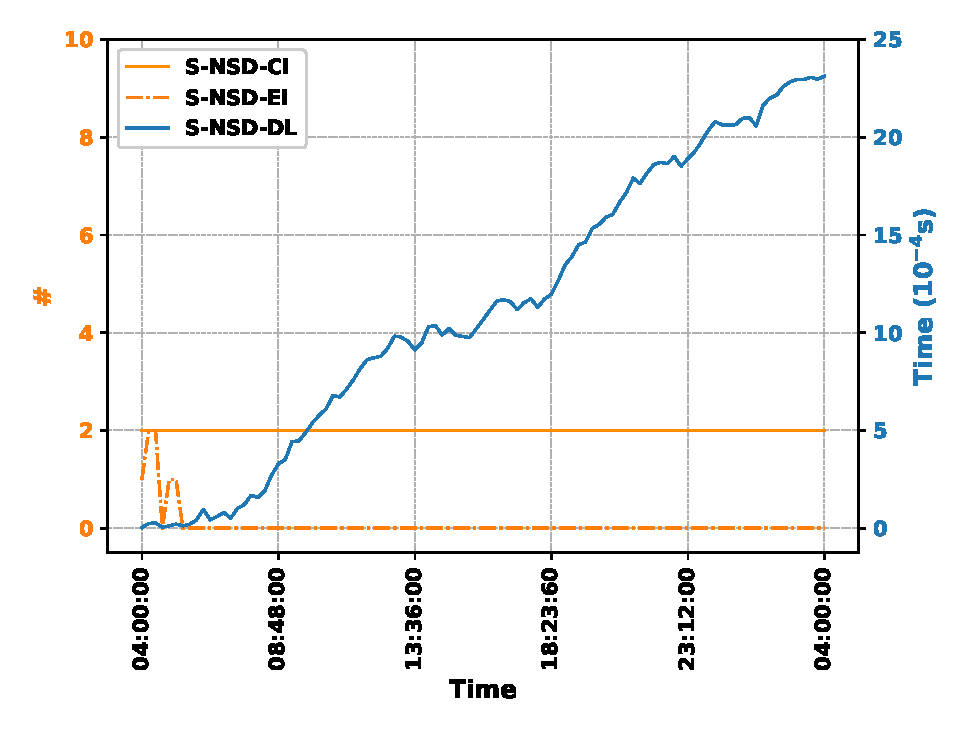
\includegraphics[width=\linewidth]{./figures/S-NSDinstance_trace.eps}
\caption{{\textsf{S-NSD}} Strategy}
\end{subfigure}
\hfill
\begin{subfigure}[h]{0.32\linewidth}
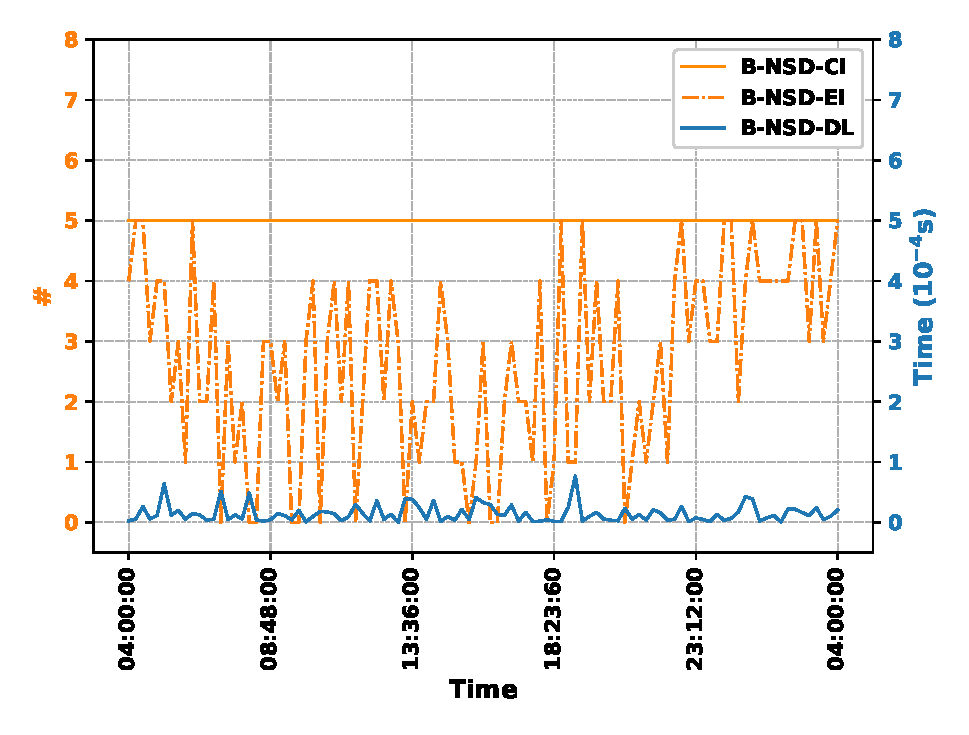
\includegraphics[width=\linewidth]{./figures/B-NSDinstance_trace.eps}
\caption{{\textsf{B-NSD}} Strategy}
\end{subfigure}
\hfill
\begin{subfigure}[h]{0.32\linewidth}
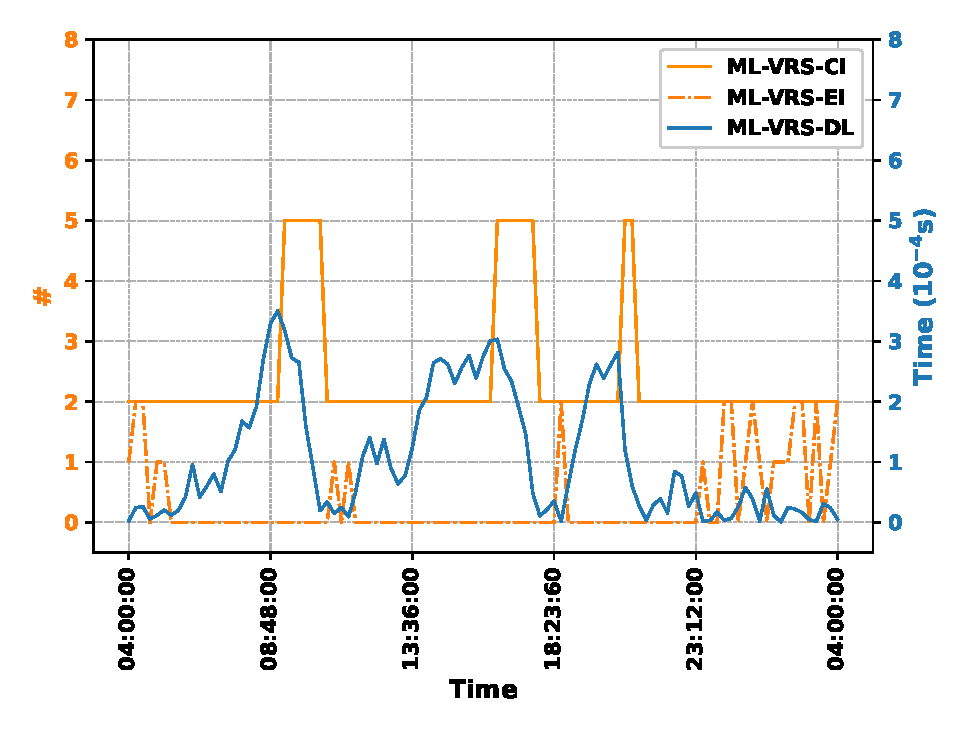
\includegraphics[width=\linewidth]{./figures/ML-VRSinstance_trace.eps}
\caption{{\textsf{ML-VRS}} Strategy}
\end{subfigure}
\caption{The traces of operation of the scaling strategies that show the number of created instances, the number of empty instances, and the processing latency.}
\label{fig:instance_trace}
\end{figure*}


\begin{figure*}
\begin{subfigure}[h]{0.32\linewidth}
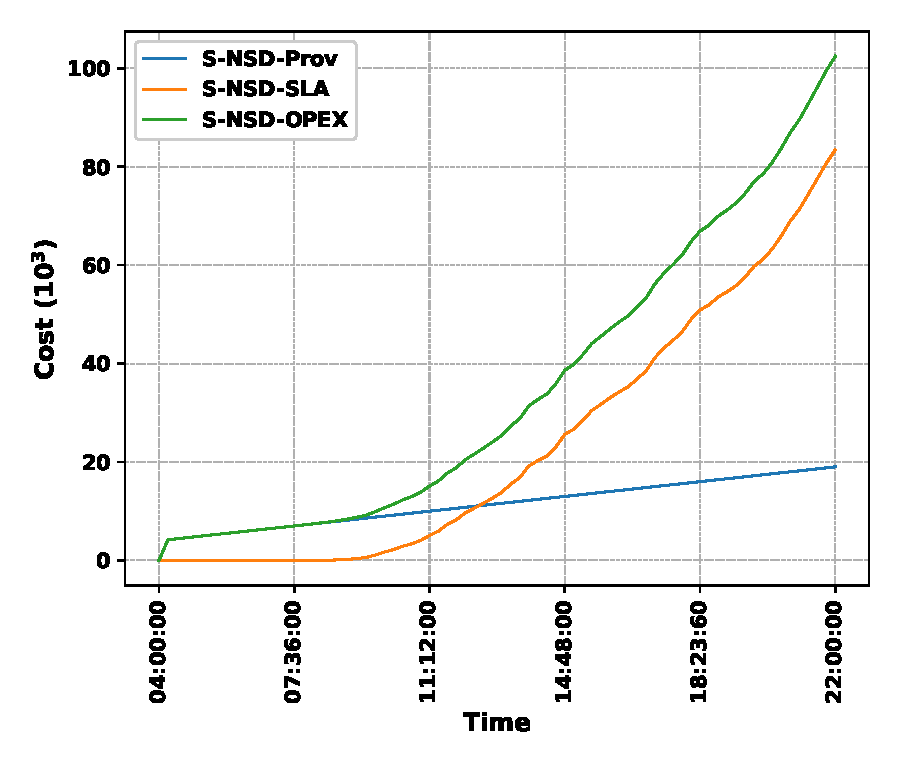
\includegraphics[width=\linewidth]{./figures/S-NSDcost_trace.eps}
\caption{{\textsf{S-NSD}} Strategy}
\end{subfigure}
\hfill
\begin{subfigure}[h]{0.32\linewidth}
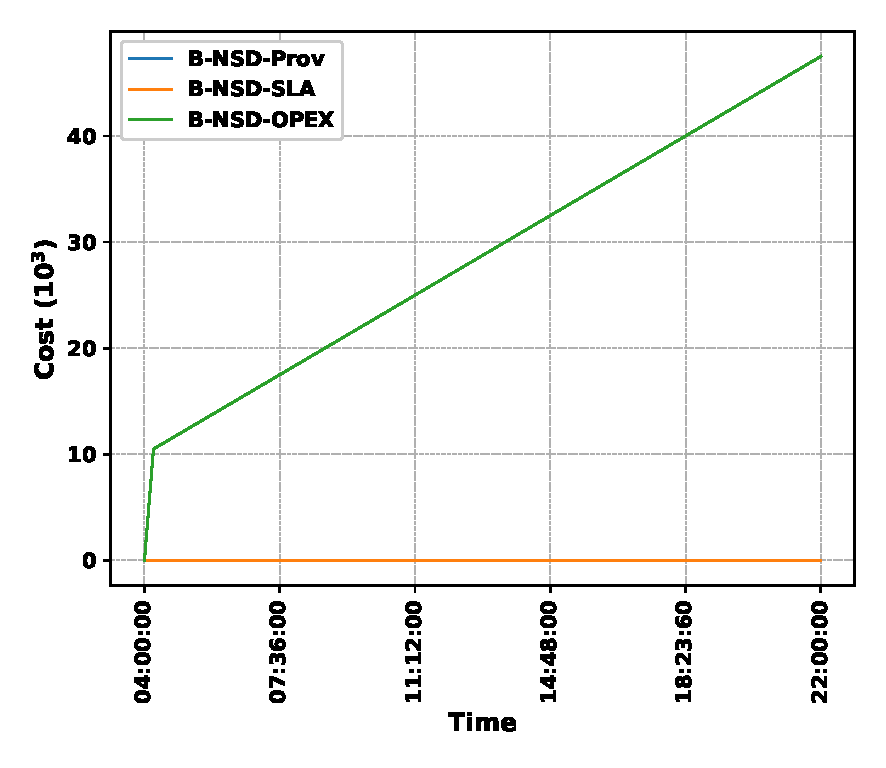
\includegraphics[width=\linewidth]{./figures/B-NSDcost_trace.eps}
\caption{{\textsf{B-NSD}} Strategy}
\end{subfigure}
\hfill
\begin{subfigure}[h]{0.32\linewidth}
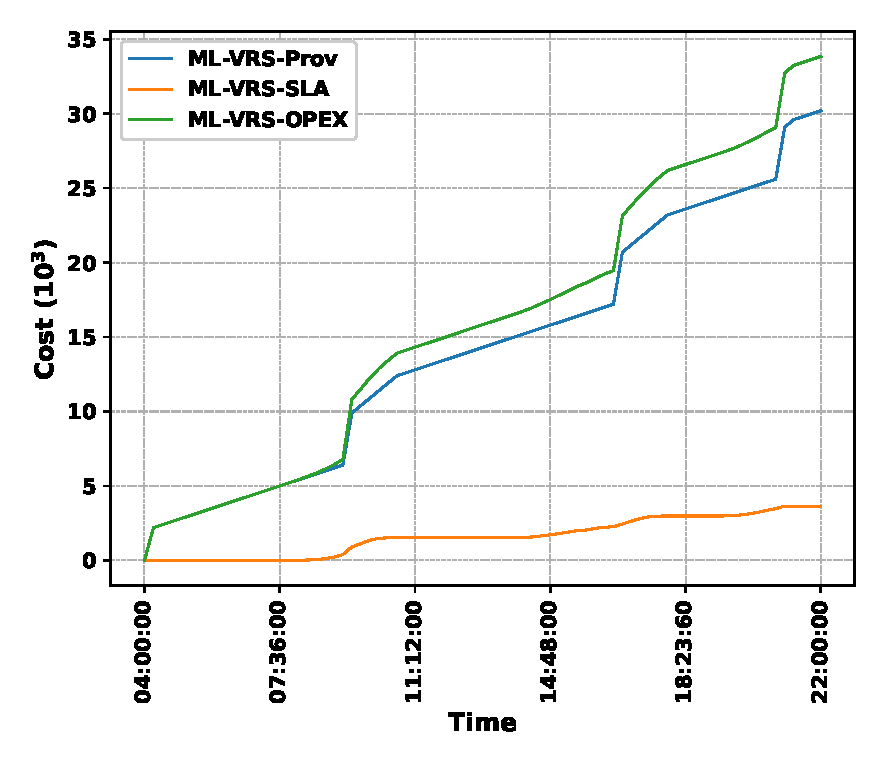
\includegraphics[width=\linewidth]{./figures/ML-VRScost_trace.eps}
\caption{{\textsf{ML-VRS}} Strategy}
\end{subfigure}
\caption{The traces of cost of the scaling strategies that show the service provisioning cost, SLA violation cost, and the OPEX.}
\label{fig:cost_trace}
\end{figure*}

To evaluate the performance of the strategies, they are compared with respect to the traffic load in Fig. \ref{fig:opex}. In these results, in each experiment, the arrival rate of the requests is multiplied by parameter $\ell$ and the total cost is computed over 24 hours period in \ref{fig:opex}-(a),(b) and over 48 hour period in \ref{fig:opex}-(c). These are the average results of 20 experiments per $\ell$. As it is shown, in the lightly loaded conditions, $\ell \leq 0.3$, all strategies comply with the SLA, so there is no SLA violation cost and because of over-provisioning, the OPEX of {\small \textsf{B-NSD}} is significant while {\small \textsf{S-NSD}} and {\small \textsf{ML-VRS}} use the minimum number of instances and have the same OPEX. By increasing $\ell$, the SLA violation cost of {\small \textsf{S-NSD}} grows exponentially but the proposed solution can maintain a negligible SLA violation by efficient resource scaling that minimizes the OPEX. In the highly loaded conditions $\ell > 1$, even the instances in the big descriptor are not sufficient to handle the offered load, so the proposed solution and the {\small \textsf{B-NSD}} has a similar performance.

To summary, these results show the superiority of the ML-driven VNF resource scaling solution to simultaneously manage the SLA of requests and minimize the OPEX. The proposed solution demonstrates how the ML-driven algorithms can be deployed via the 5Growth platform.   


\begin{figure*}
\begin{subfigure}[h]{0.32\linewidth}
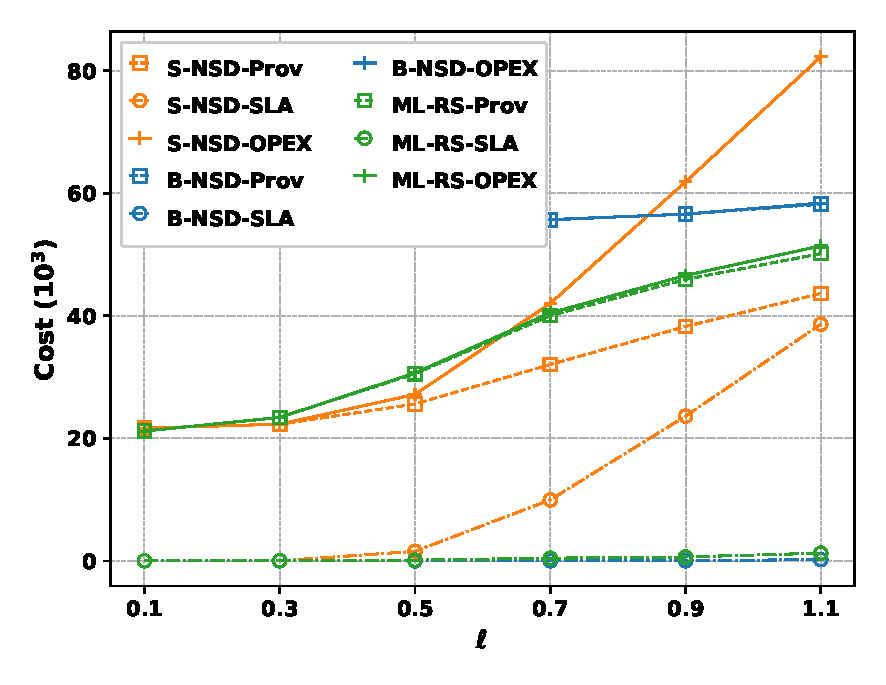
\includegraphics[width=\linewidth]{./figures/Automative.eps}
\caption{Collision Detection services in a 24 hour period}
\end{subfigure}
\hfill
\begin{subfigure}[h]{0.32\linewidth}
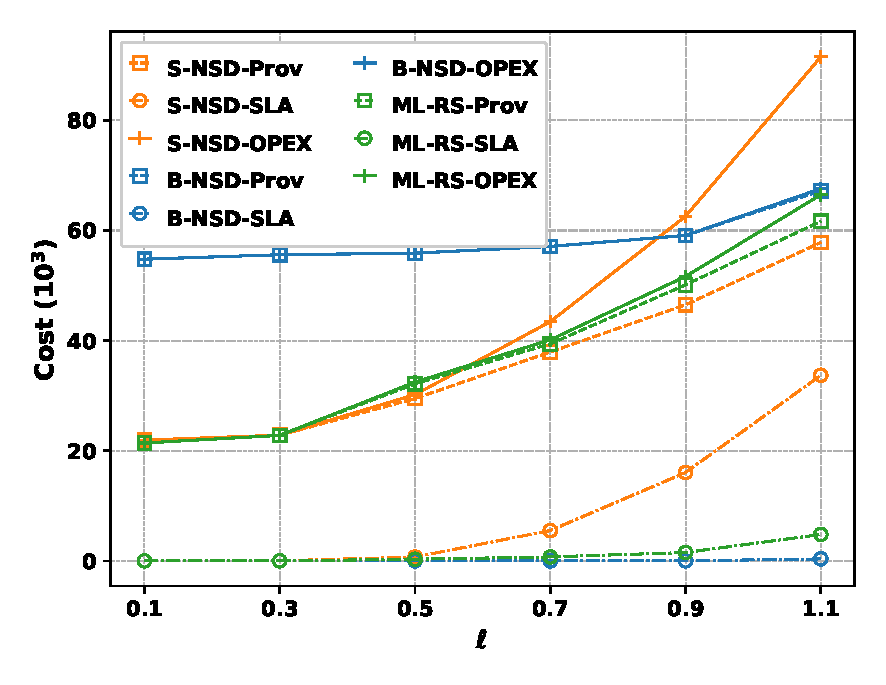
\includegraphics[width=\linewidth]{./figures/bird_eye.eps}
\caption{Bird Eye service in a 24 hour period}
\end{subfigure}
\hfill
\begin{subfigure}[h]{0.32\linewidth}
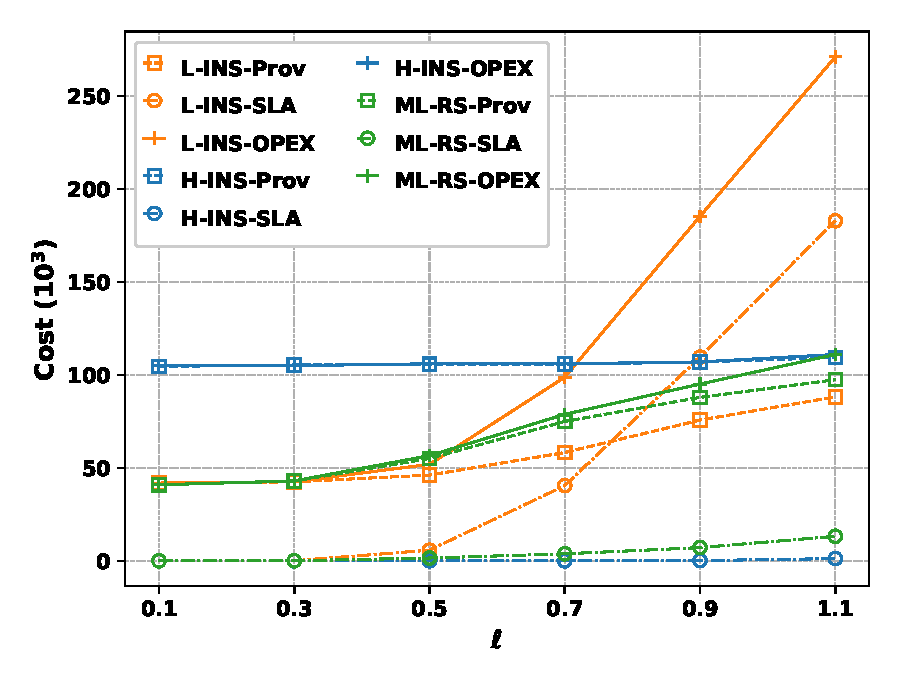
\includegraphics[width=\linewidth]{./figures/bird_eye-2days.eps}
\caption{Bird Eye service in a 48 hour period}
\end{subfigure}
\caption{The Provisioning cost, SLA violation cost and the OPEX with respect to the scale of the arrival rate of the requests.}
\label{fig:opex}
\end{figure*}

\begin{figure*}
\begin{subfigure}[h]{0.32\linewidth}
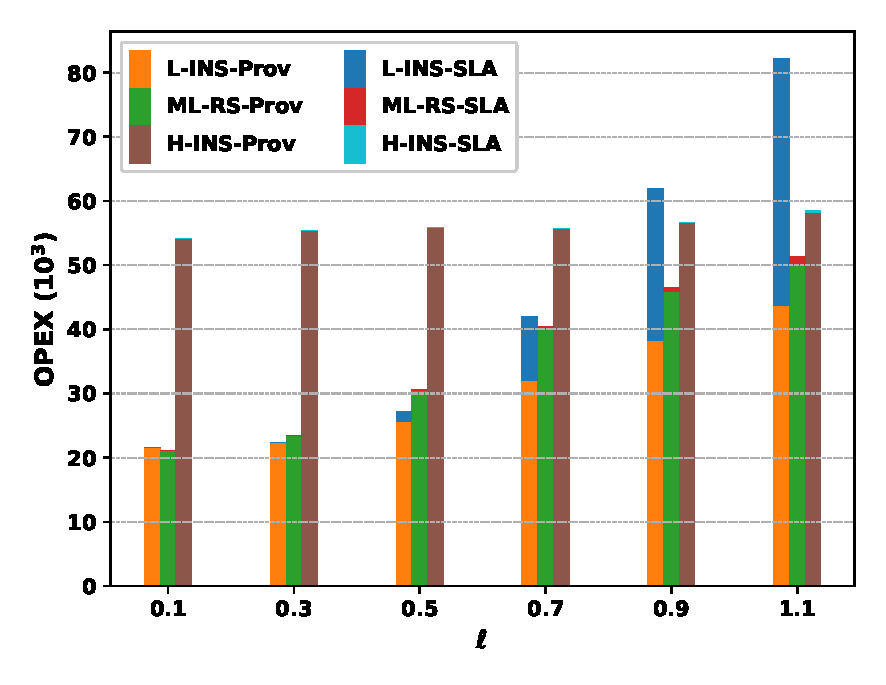
\includegraphics[width=\linewidth]{./figures/Automative-bar.eps}
\caption{Collision Detection services in a 24 hour period}
\end{subfigure}
\hfill
\begin{subfigure}[h]{0.32\linewidth}
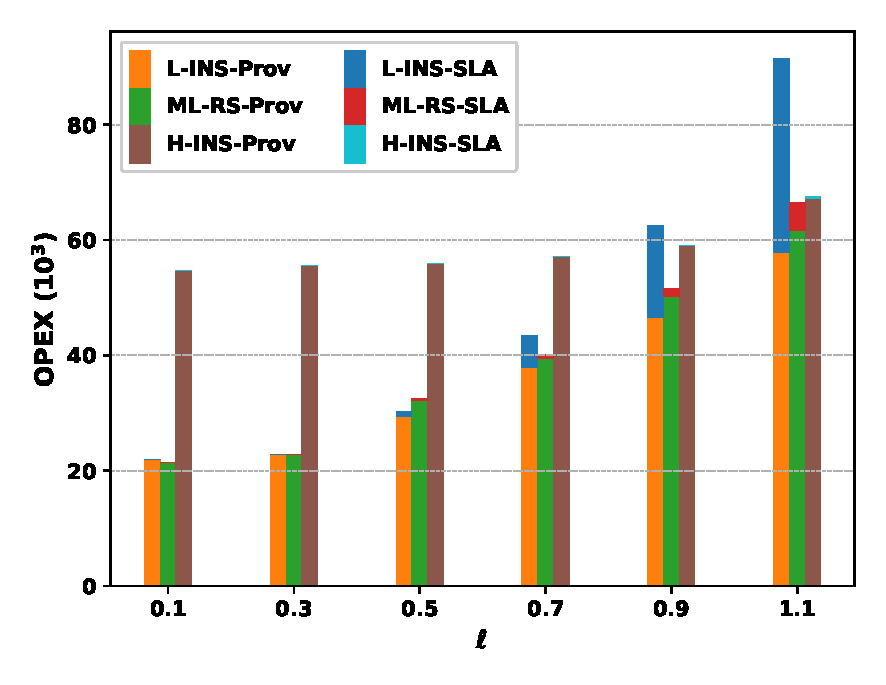
\includegraphics[width=\linewidth]{./figures/bird_eye-bar.eps}
\caption{Bird Eye service in a 24 hour period}
\end{subfigure}
\hfill
\begin{subfigure}[h]{0.32\linewidth}
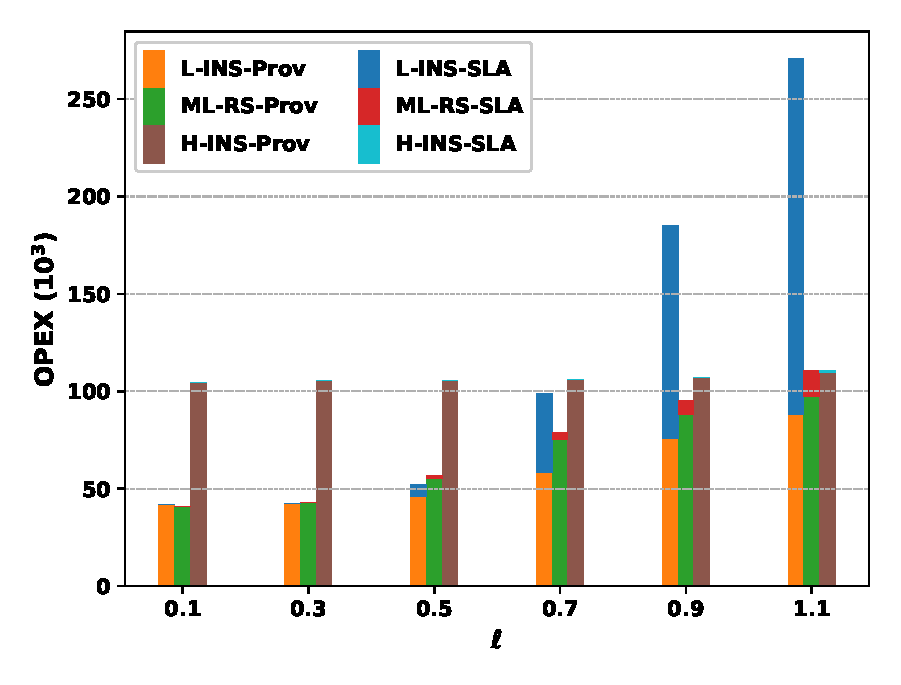
\includegraphics[width=\linewidth]{./figures/bird_eye-2days-bar.eps}
\caption{Bird Eye service in a 48 hour period}
\end{subfigure}
\caption{The Provisioning cost, SLA violation cost and the OPEX with respect to the scale of the arrival rate of the requests.}
\label{fig:opex}
\end{figure*}

} % end of \hlb


\end{document}
